\documentclass[twocolumn,a4paper]{article}
\usepackage{graphicx}
\usepackage{amsfonts}
\usepackage{color}
\usepackage{lineno}
\setlength{\columnsep}{10pt}
\setlength{\oddsidemargin}{0pt}
\setlength{\topmargin}{0pt}
\setlength{\headheight}{0pt}
\setlength{\headsep}{0pt}
\setlength{\marginparsep}{0pt}
\setlength{\marginparwidth}{0pt}
\addtolength{\voffset}{-50pt}
\setlength{\textheight}{26.8cm}
\author{Siwang Li}

\title{Implementation of Material Optimization}

%% document begin here
\begin{document}
\maketitle

\section{Input Animation}
The motion equation of one mode is
\begin{equation} \label{deeq}
  \ddot{z} + (\alpha_m+\alpha_k\lambda)\dot{z} + \lambda z = 0
\end{equation}
and the analytical solution of $z(t)$ is
\begin{equation} \label{oss}
  z(t) = (Pcos(wt) + Qsin(wt))e^{-\alpha t}
\end{equation}
where the angular velocity is defined as $w = \sqrt{\lambda-\alpha^2}$, the
decay rate $\alpha = (\alpha_k\lambda+\alpha_m)/2$, and $P$ and $Q$ are
arbitrary scalar values depicting the initial amplitude and phase of this mode,
\begin{eqnarray}\label{PQ}
  P &=& z(0) \\
  Q &=& \frac{1}{w}(\dot{z}(0) + \alpha z(0))
\end{eqnarray}
In the following experiments, we use $z(t)$ to produce the animation sequence
using single or multiple modes, then use them to fit the elastic materials.

\section{Approximate Materials}
Given the input sequence $z_0,\cdots,z_T$, we define a quadratic energy function
\begin{equation} \label{qua-en}
  E(k,d) = \sum_{i=2}^{T-1} \|\frac{1}{h^2}\hat{z}_i+\frac{1}{h}\hat{D}(d)(z_{i+1}-z_{i})+ K(k)z_i\|_2^2
\end{equation}
where $h$ is the time step,$\hat{z}_i=z_{i+1}-2z_{i}+z_{i-1}$,$\hat{D}(d) =
diag(d_1,\dots,d_m)$ is a diagonal matrix represent the damping, and $K(k)$ is a
dense symmetric matrix which is obtained by properly assemble $k_i$ into
$K$. Firstly, we will suppose $\hat{D}$ is known, and optimize for $K$
only. Then we try to optimize for both $K$ and $D$.

\section{Results}
In the first experiment, we produce the animation of a single mode with
$\lambda=0.5,\alpha_k=\alpha_m=0,T=500,h=0.1,z(0)=0.5,\dot{z}(0)=0.8$. The
residual $|k-\lambda|/\lambda=4.1\times 10^{-4}$, $E(\lambda)=1.6\times
10^{-5}$, and $E(k)=4\times 10^{-23}$. We use $\lambda$ and $k$ in (\ref{oss})
to obtain two motion curves of $z$, and we record them as $z(t,\lambda)$ and
$z(t,k)$ respectively. We draw curves of these two functions, and found them
almost the same(see figure \ref{singleModeNoCon}). We also found that the
initial speed $\dot{z}(0)$ also has no impact on fitting $k$.
\begin{figure}
  \centering
  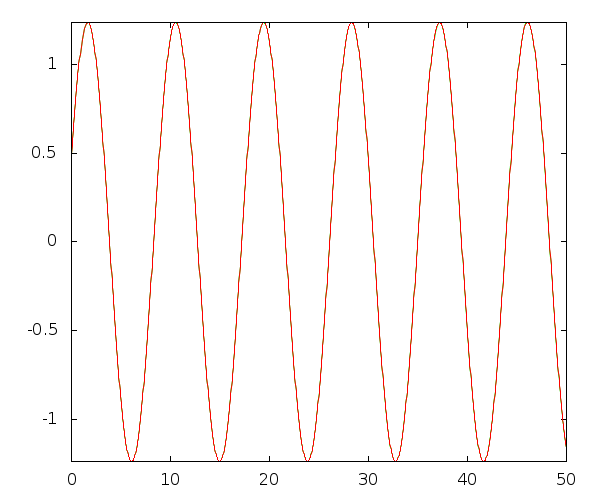
\includegraphics[width=0.4\textwidth]{./figures/singleModeNoDamp.png}
  \caption{Blue is $z(t,\lambda)$, and red is $z(t,k)$, they are overlapped.}
  \label{singleModeNoCon}
\end{figure}

In the second experiment, we use damping to produce the input animation with
$\alpha_k=\alpha_m=0.5$, and other parameters are same as above. We set
$\hat{D}=0$ and $\hat{D} = \alpha_k\lambda+\alpha_m$ respective to optimize for
$k$. The resulting curves are shown in figure \ref{singleModeD}. It obvious that
when damping are considered in the fitting process, the results will be better.
\begin{figure}
  \centering
  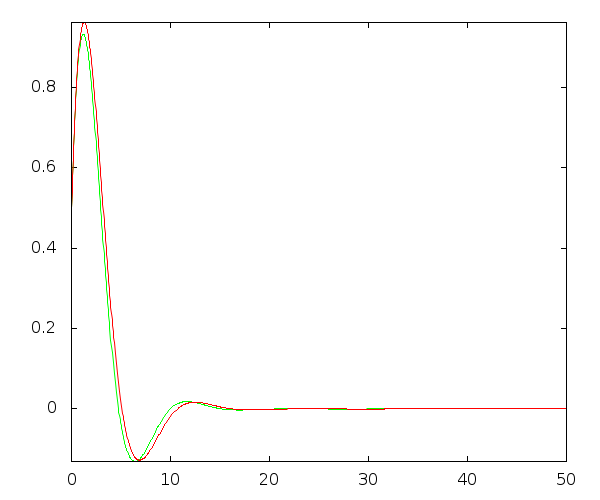
\includegraphics[width=0.24\textwidth]{./figures/singleModeD0.png}
  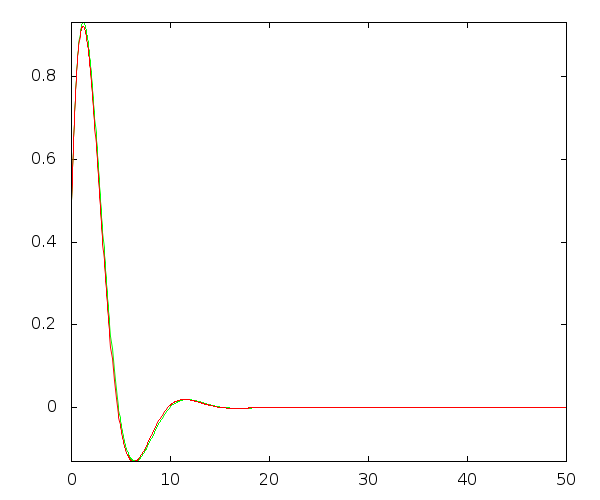
\includegraphics[width=0.24\textwidth]{./figures/singleModeD.png}
  \caption{Left is $\hat{D}=0$, and right is
    $\hat{D}=\alpha_k\lambda+\alpha_m$. In both pictures blue is $z(t,\lambda)$,
    and red is $z(t,k)$.}
  \label{singleModeD}
\end{figure}

In the third experiment, we use the same setting as above to produce the input
animation, and this time, we optimize for both $d$ and $k$ simultaneously.

% \subsection{Experiments}
% \begin{itemize}
% \item Use an random vector $x$ to check $E(x)-(\frac{1}{2}x^THx+b^Tx+E(0))$ to
%   make sure $H$ and $b$ are correct.({\color{red}result $<10^{-10}E(x)$}).
% \item Check $Hk = -b$ to make sure the equation solving is
%   correct({\color{red}result $<10^{-8}$}).
% \item We use a single mode (eigenvalue $\lambda=0.5$) to produce the animation
%   $z'_1,\cdots,z'_{100}$ with a RS simulator without constraints. Implicit
%   integration method is used. Then we use it to produce $K\in R^{1\times1}$. We
%   check the residual $|\frac{K}{\lambda}-1|$,$E(\lambda)$, and
%   $E(k)$. ({\color{red}the values are 0.01,4.618,4.515. $E(\lambda)$ is not
%     zero, because the descrete scheme in equation (\ref{qua-en}) is actually not
%     equal to an implicit integration.}).
% \item Use different time step $h$ to make the above
%   experiment. ({\color{red}when $h$ become larger, the residual $E(k)$ become
%     smaller. Suppose $\zeta$ is the scalor for $h$, then $E(k,\zeta h) =
%     \frac{E(k,h)}{\zeta^4}$}.)
% \item We use the first 20 modes to produce the animation $z'_0,\cdots,z'_{T}$
%   with a RS simulator without constraints, then use it to compute $K$. We check
%   the residual $E(k)$. ({\color{red}We choose different $T=10,20,50,100$, and
%     the corresponding residuals are $E(k)=1.63,23.08,281.5,400$})
% \item Make a similar experiment as above, but with some nodes are
%   constrained. There is no need to introduce additional constraint forces into
%   to (\ref{qua-en}), as we constrained the nodes during the modal analysis
%   process by removing the corresponding columns and rows from the stiffness and
%   mass matrix. ({\color{red}We choose different $T=10,20,50,100$, and
%     the corresponding residuals are $E(k)=0.8,10.47,187.4,285.9$})
% \item Produce $z'$ of only one mode ($\lambda = 0.5$) without damping using
%   analysis simulator $z(\lambda,t)$. Print the two curves $z(\lambda,t)$ and
%   $z(k,t)$, check $E(\lambda)$ and $E(k)$.
% \item Make the same experiment as above, but introduce damping to produce $z(t)$
%   and use the same damping in $E(k)$ to compute $k$.
% \item Make the same experiment as above, but the damping in $E(k)$ is set as
%   unknowns.
% %% \item Use different time step $h$ to make the above experiment.
% %% \item We use a full StVK simulator to produce an animation $P =
% %%   (p_1,\cdots,p_T)$ without constraints. Then compute $K$ and check the residual
% %%   $E(k)$.
% %% \item Use different time step $h$ to make the above experiment.
% %% \item Use the same $P$ as above, but compute $z' = \hat{W}^{-1}\hat{P}$. Check
% %%   the residual $E(\Lambda)$.
% %% \item Use same $z'$ as above, compute $K$, check the residual $E(k)$.
% %% \item Produce all the input and out animation, check the deformation results and
% %%   dynamics.
% \end{itemize}

% \subsection{Conclusion}
% Firstly, because the discrete scheme in equation (\ref{qua-en}) is not equal to
% an implicit integration. Thus if the animation is produced by using an implicit
% simulator, the real elastic material can not satisfy $E(k)=0$. Secondly, large
% time step will result in small residual $E(k)$. Thirdly, larger $T$ will result
% in larger residual $E(k)$. This is because we use the quadratic objective
% (\ref{qua-en}) to minimize the residual of $r\times T$ linear equations, with
% unknowns of $r\times r$.

% \section{Analysis Results}


% %% references
% % \begin{thebibliography}{99}
% % \bibitem{sig2011} Fast simulation of skeleton-driven deformable body
% %   characters.
% % \end{thebibliography}

\end{document}
